\section{Appendices}

\begin{figure*}[]
    \centering
    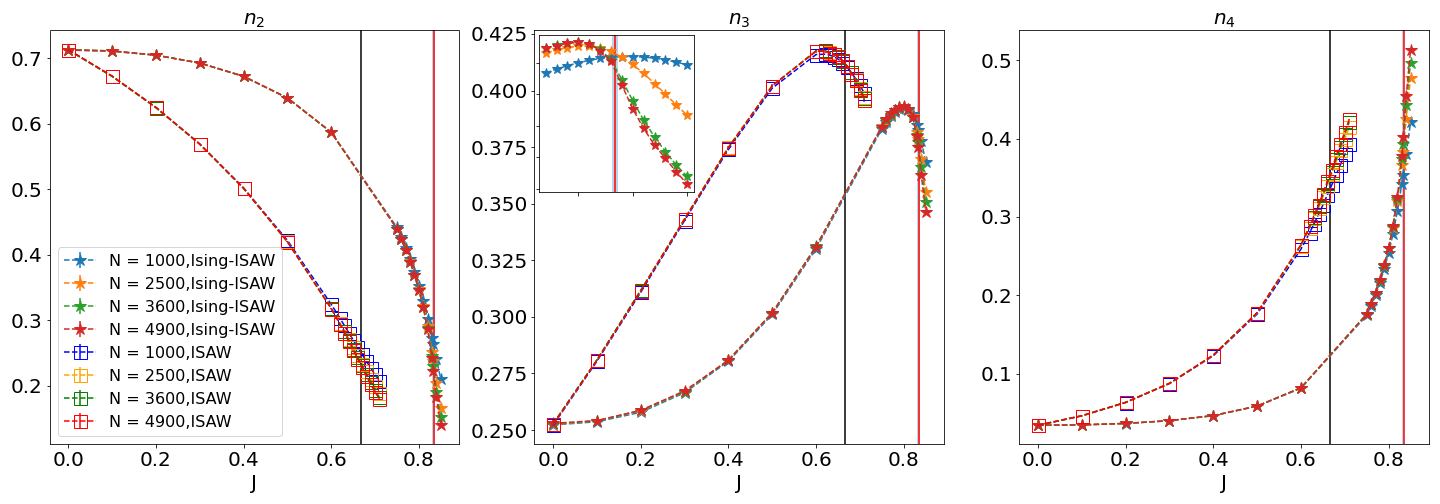
\includegraphics[width=0.99\textwidth]{Images/bulk2-4_inset.png}
    \caption{Fractions of monomers of Ising-ISAW model (squares) and ISAW model (stars) on a square lattice with 2-4 nearest neighbors as function of $J$ with length of conformations $N = $ 1000 (blue), 2500 (yellow), 3600 (green), 4900 (red). Black vertical line define point of $\theta$-transition for ISAW model \cite{Caracciolo2011}, red line - for Ising-ISAW model \cite{faizullina2021critical, Foster2021}. Reproduced from Ref.\cite{faizullina2021critical}}
    \label{fig:Ising_vs_ISAW2D}
\end{figure*}


\begin{figure*}[]
    \centering
    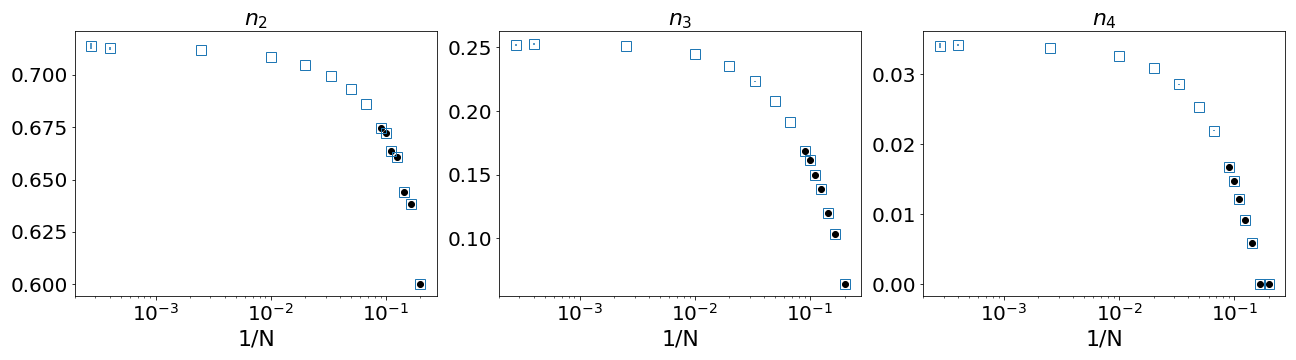
\includegraphics[width=0.99\textwidth]{Images/ISAWJ0_Bulk2-4.png}
    \caption{Fractions of monomers of ISAW model on a square lattice with 2-4 nearest neighbors at $J=0$ as function of $1/N$, from $N = 5$ to $3600$ for MC simulations (empty squares) and from $N = 5$ to $11$ for enumerations (black dots)}
    \label{fig:Ising_vs_ISAW}
\end{figure*}

\begin{figure*}
    \centering
    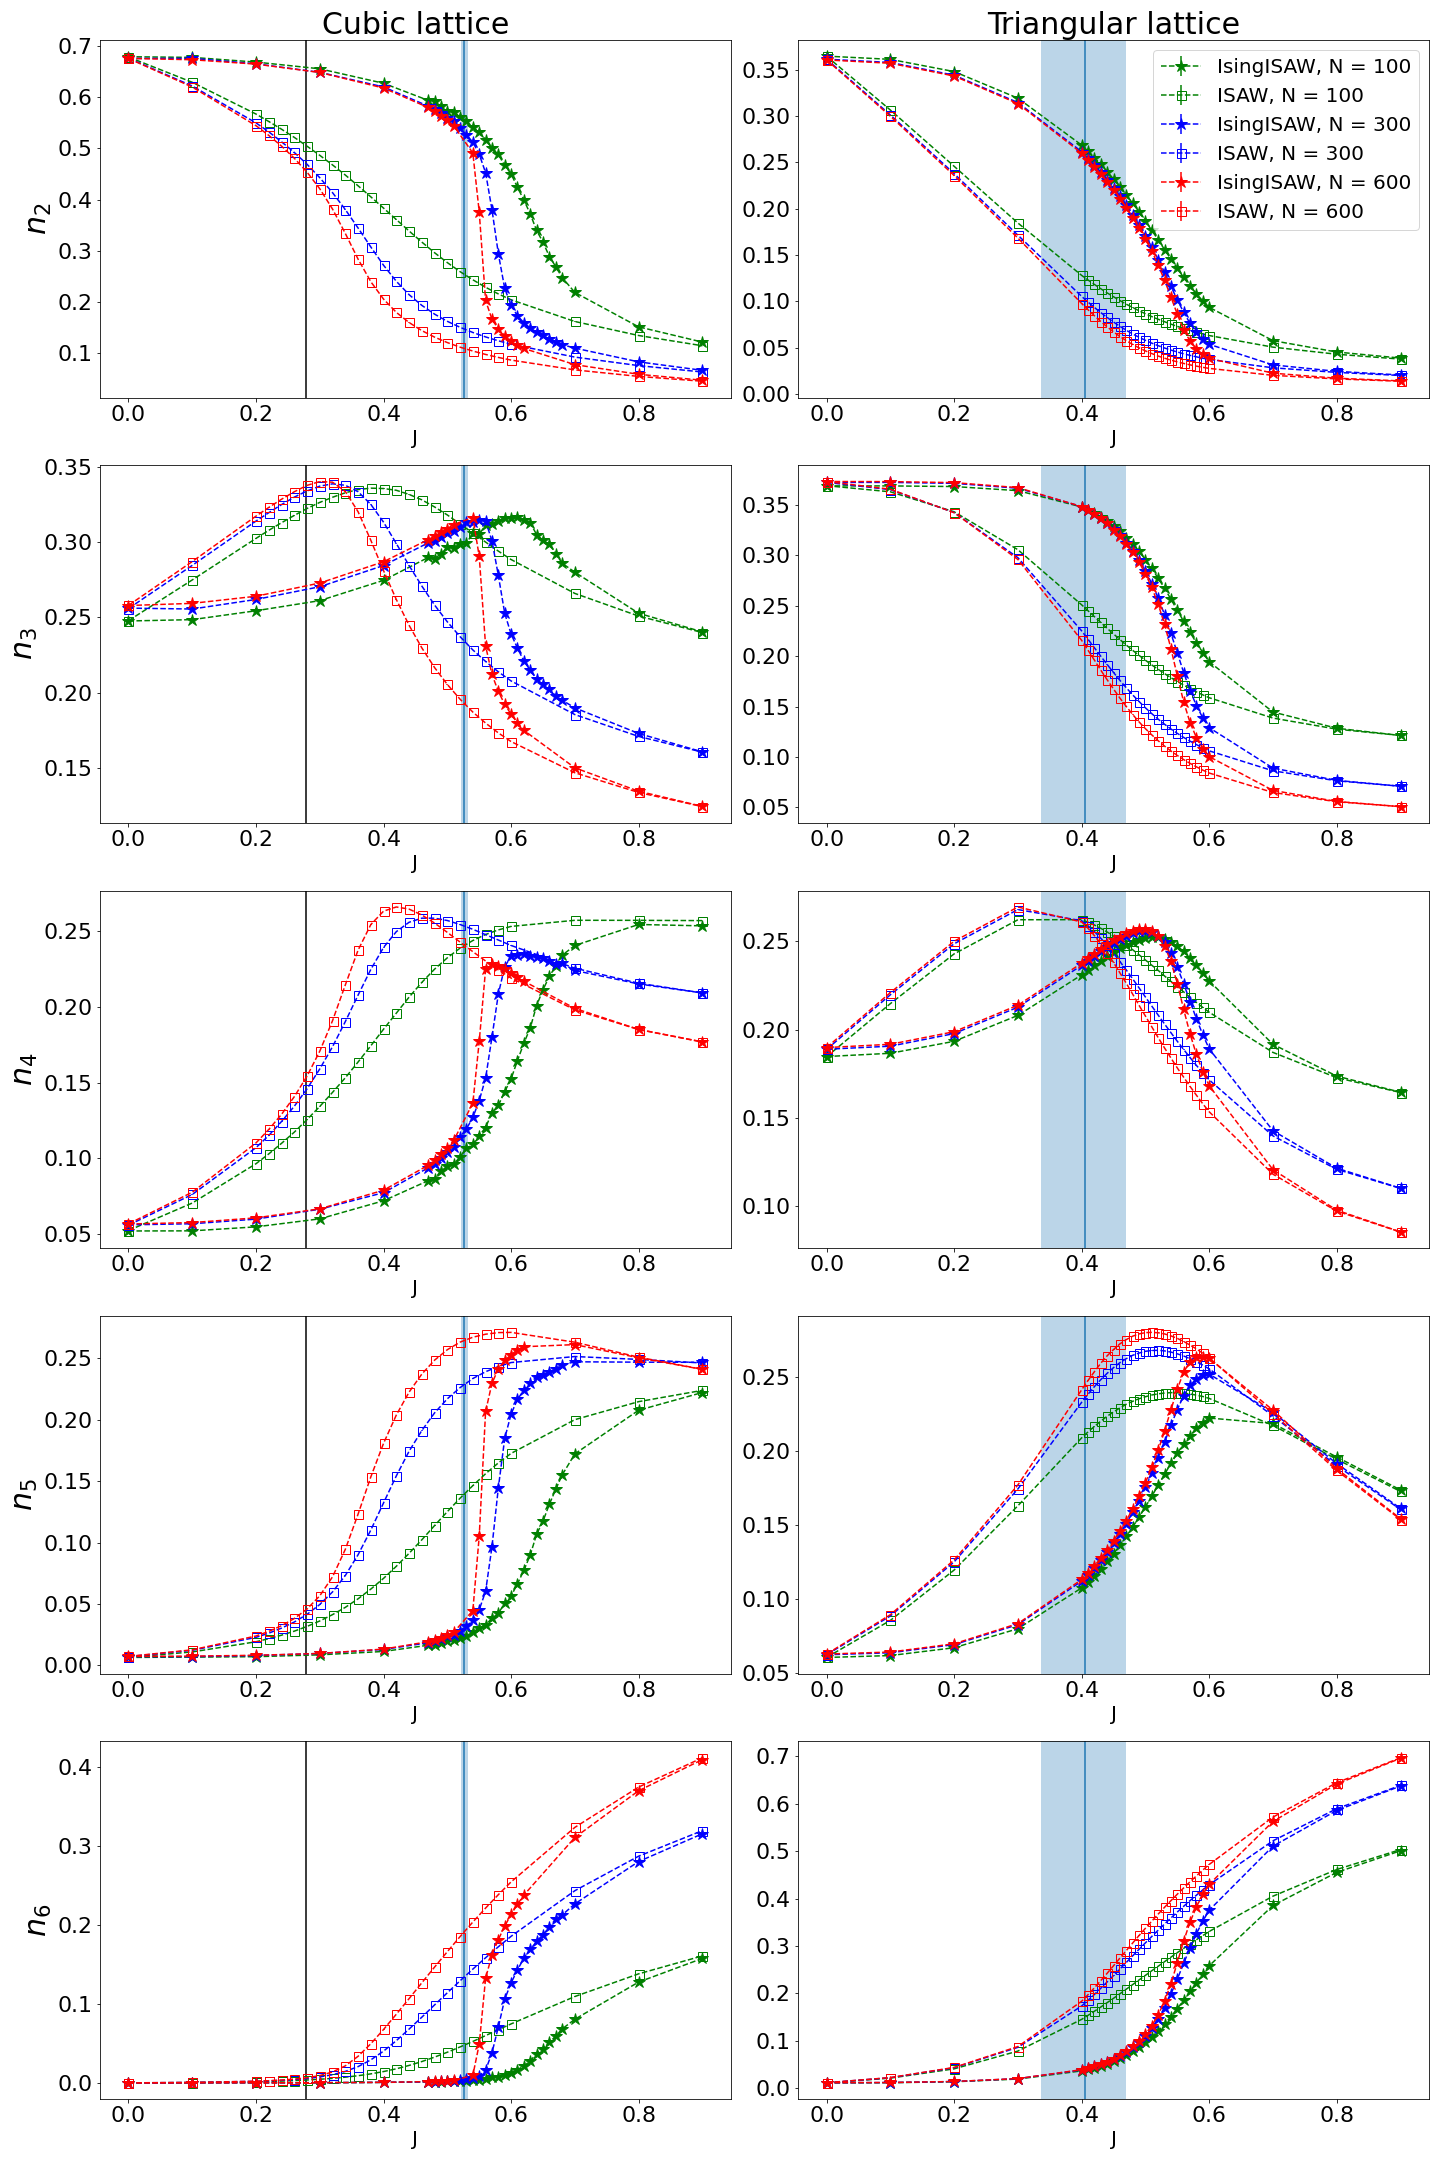
\includegraphics[width=0.95\textwidth, height=22.5cm]{Images/Ising_vs_ISAW.png}
    \caption{Fractions of monomers of Ising-ISAW model (stars) and ISAW model (open squares) on a cubic lattice (left column) and 2D-triangle lattice (right column) with 2-6 nearest neighbors as function of $J$ with length of conformations $N = $ 100 (green), 300 (blue) and 600 (red). Vertical lines define points of $\theta$-transition (For cubic lattice: black line for ISAW model \cite{Tesi1996} and blue line for Ising-ISAW model \cite{Foster2021}; for triangle lattice: blue line for ISAW model \cite{Privman1986})}
    \label{fig:Ising_vs_ISAW}
\end{figure*}